\documentclass{beamer}

\usefonttheme{professionalfonts} % using non standard fonts for beamer
\usefonttheme{serif} % default family is serif

\usepackage{hyperref}
%\usepackage{minted}
\usepackage{animate}
\usepackage{graphicx}
\def\Put(#1,#2)#3{\leavevmode\makebox(0,0){\put(#1,#2){#3}}}
\usepackage{colortbl}
\usepackage{tikz}
\usepackage{amssymb}
\usepackage{enumerate}
\usepackage{arydshln}
\usepackage{algorithm}
\usepackage{algpseudocode}

\colorlet{lightred}{red!25}
\colorlet{lightgreen}{green!25}


\newcommand\blfootnote[1]{%

  \begingroup

  \renewcommand\thefootnote{}\footnote{#1}%

  \addtocounter{footnote}{-1}%

  \endgroup

}

\makeatletter

%%%%%%%%%%%%%%%%%%%%%%%%%%%%%% Textclass specific LaTeX commands.

 % this default might be overridden by plain title style

 \newcommand\makebeamertitle{\frame{\maketitle}}%

 % (ERT) argument for the TOC

 \AtBeginDocument{%

   \let\origtableofcontents=\tableofcontents

   \def\tableofcontents{\@ifnextchar[{\origtableofcontents}{\gobbletableofcontents}}

   \def\gobbletableofcontents#1{\origtableofcontents}

 }

%%%%%%%%%%%%%%%%%%%%%%%%%%%%%% User specified LaTeX commands.

\usetheme{Malmoe}

% or ...

\useoutertheme{infolines}

\addtobeamertemplate{headline}{}{\vskip2pt}

\setbeamercovered{transparent}

% or whatever (possibly just delete it)

\makeatother

\begin{document}
\title[PFLOCK report]{PFLOCK Report}
\author[AC]{Andres Calderon}
\institute[Winter'20]{University of California, Riverside}
\makebeamertitle
\newif\iflattersubsect

\AtBeginSection[] {
    \begin{frame}<beamer>
    \frametitle{Outline} 
    \tableofcontents[currentsection]  
    \end{frame}
    \lattersubsectfalse
}

\AtBeginSubsection[] {
    \begin{frame}<beamer>
    \frametitle{Outline} 
    \tableofcontents[currentsubsection]  
    \end{frame}
}

\begin{frame}{About indexing...}
    \begin{itemize}
        \item GeoSpark makes partitioning and indexing in a \textbf{SpatailRDD} in two diferent stages:
        \begin{enumerate}
            \item Once a partitioner (Quadtree, KDBtree, ...) is created, a \textbf{SpatialRDD} call \texttt{partition} method to move data to the corresponding partition (it use the \texttt{partitionBy} method of Apache Spark).
            \item Given a \textbf{SpatialRDD} already partitioned you can call \texttt{buildIndex} method which make a call to the \texttt{IndexBuilder} class (it will create a Quadtree or Rtree in the data of each partition).
        \end{enumerate}
        \item Feeding the index at the moment the data is moved would demand modification of Apache Spark code...
    \end{itemize}
\end{frame}

\begin{frame}{About Join...}
    \begin{itemize}
        \item GeoSpark provides two types of joins:
    \end{itemize}
    \centering
    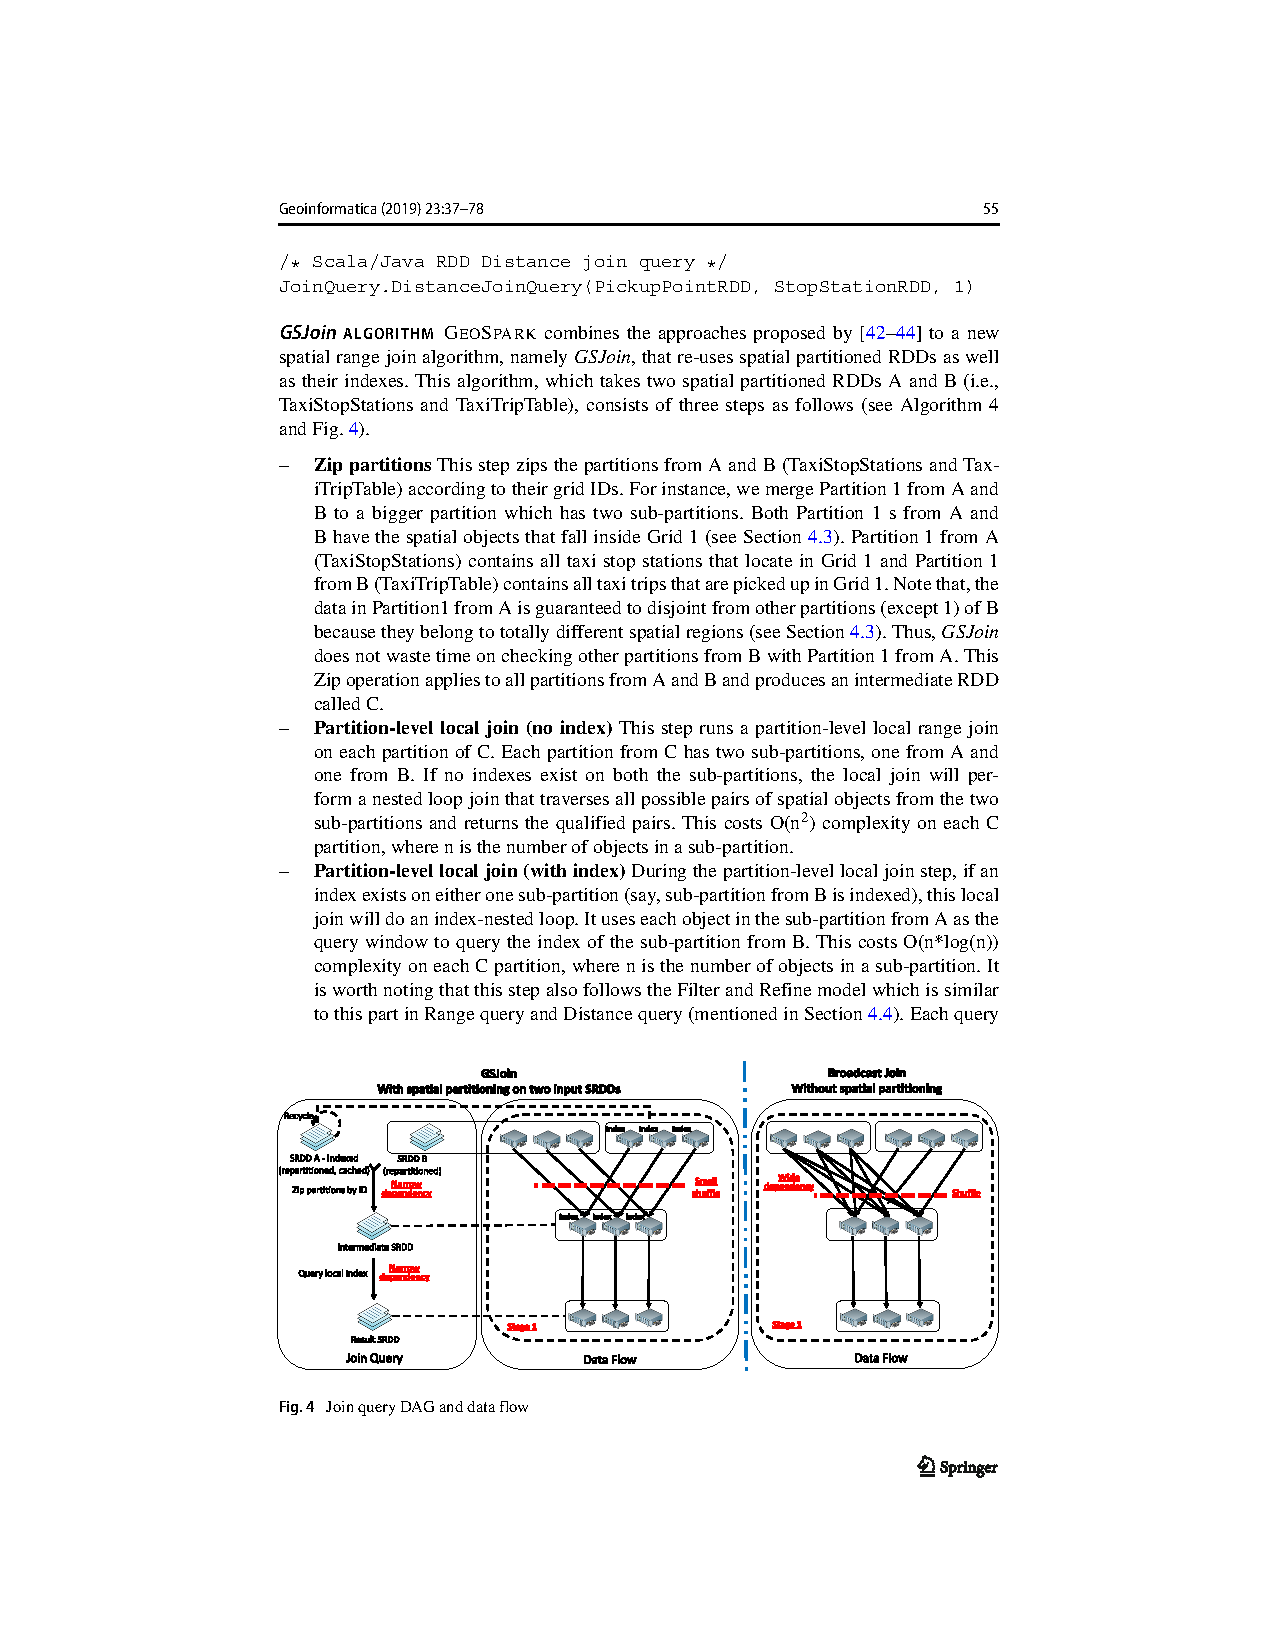
\includegraphics[trim=4.0cm 4.5cm 4.0cm 18.0cm, clip, width=1\textwidth]{figures/joins}
\end{frame}

\begin{frame}{About Join...}
    \begin{itemize}
        \item GSJoin is actually a combination of Index-based and Nested-loop joins:
        \begin{enumerate}
            \item If one of the SpatialRDDs is indexed, it will query that index to get a set of candidates and then refine the search.
            \item If no index is present, it will run a nested loop join.
        \end{enumerate}
        \item By default, GSJoin uses left OR right index but not both...
    \end{itemize}
\end{frame}

\begin{frame}{About Join...}
    \begin{itemize}
        \item GSJoin performs some verifications which are not needed for distance joins involving Point datasets (CRS and partition matches, statistic collection ).
        \item I have been able to port the code to Scala and remove unnecesary verifications.  
        \item It saves $\approx1.5$s but still have to perform more robust tests.
        \item Currently checking the merge operation to see if they are using just the data in the border of the partition...
    \end{itemize}
\end{frame}

\end{document}
